%
% Umsetzung
%
\chapter{Umsetzung}
\label{cap-umsetzung}
Dieser Abschnitt beschreibt die technischen Hilfsmittel und Vorgehensweisen bei der Umsetzung der Projektidee.
Die Architektur kann in drei Bereiche geteilt werden.
Zuerst werden die Daten aus verschiedenen Quellen zusammengetragen, aufbereitet und in dem zentralen Triplestore gespeichert. (Siehe \ref{design-step11})
Der zweite Bereich beschäftigt sich damit, wie die semantischen Daten der Welt zugänglich gemacht werden.
Zuletzt wird die Beispielanwendung ``Semantic Internship Advisor'' vorgestellt, welcher auf die Daten zugreift.
\section{Architektur Übersicht}

\begin{figure}[h]
	\centering
	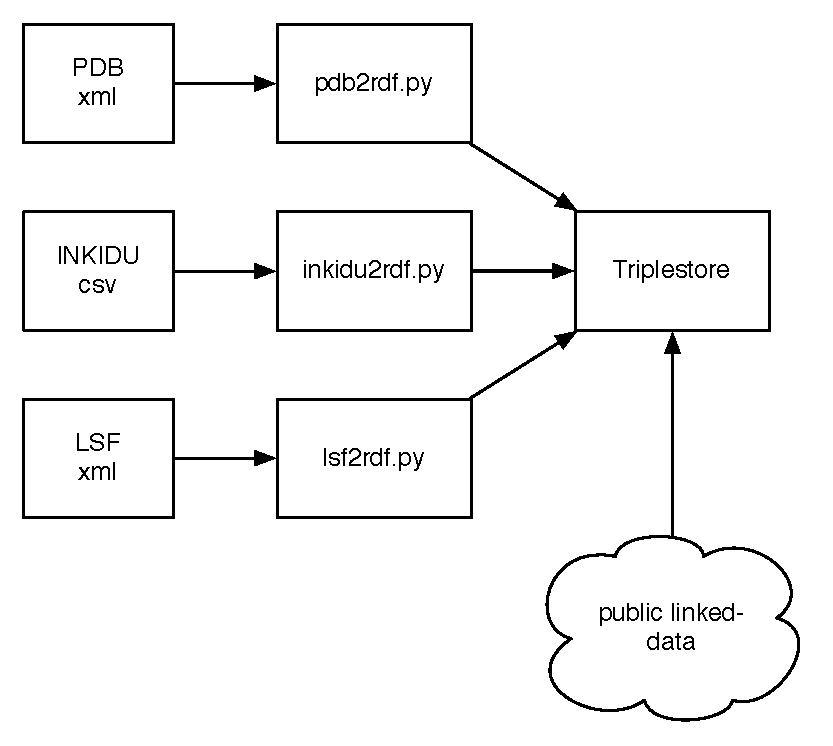
\includegraphics[scale=0.6,]{images/step1_1.pdf}
	\caption{Architektur: Daten aufbereiten}
	\label{design-step11}
\end{figure}

\section{Daten aufbereiten: Python Skripte} %wiedi
\label{sec-daten-python}
Die Konvertierung der Datenquellen nach RDF ist mit Hilfe von drei kleinen Python Skripten umgesetzt.
Für jede Datenquelle wurde ein Skript verfasst.


\subsection{RDFLib}
\label{subsec-rdflib}
Dank RDFLib\footnote{\url{http://www.rdflib.net/}} ist das Erstellen eines Graphen und die Ausgabe als RDF/XML sehr einfach zu realisieren.
RDFLib ist eine Python Bibliothek, welche Parser und Serialisierer für viele Varianten von RDF enthält.
Des weiteren ist ein ``in-memory'' Graphstore enthalten. Es besteht aber ebenso die Möglichkeit den Graphen persistent zu speichern.

\subsection{Arbeitsweise}
Die Skripte arbeiten in zwei schritten.
Im ersten Schritt werden die Originaldaten geladen und in eine interne Datenstruktur gebracht.
Für XML Quellen wird das Python Modul ">xml.dom.minidom"< als Parser eingesetzt.
Für das CSV Format bietet Python in seiner Standardbibliothek einen Parser.

Im zweiten Schritt wird die Datenstruktur abgearbeitet und in Triples strukturiert.
Diese Triples werden dann in einen temporären Graphen eingefügt.

\begin{lstlisting}[language=Python,caption=Alle Betreuer einer Firma werden zum Graphen ``g'' hinzugefügt,stepnumber=1,label=umsetzung-rdflib-add]
for betreuer in firma['betreuer']:
	betreuer_node = PDB_BETREUER[betreuer['id']]
	g.add((betreuer_node, RDF.type, FOAF['Person']))
	g.add((betreuer_node, FOAF['member'], firma_node))
	g.add((betreuer_node, FOAF['name'], Literal(betreuer['name'])))
\end{lstlisting}

Im Codelisting \ref{umsetzung-rdflib-add} wird für jeden Betreuer einer Firma eine ``betreuer\_node'' im Namespace PDB\_BETREUER erstellt.
Über diese Node werden dann drei Aussagen (Triples) getroffen. Zuerst wird der Typ als foaf:Person festgelegt.
In Zeile 4 wird festgelegt, dass der Betreuer Mitglied einer Firma ist. Zuletzt wird der Name als Literal gesetzt.
Diese drei Aussagen werden in den Graphen ``g'' mit der ``add'' Methode hinzugefügt.

\subsection{Verknüpfen der Datenquellen}

In dem Umfragetool INKIDU werden die Firmen einzig über ein Freitextfeld identifiziert, welches vom Umfrageteilnehmer ausgefüllt wird.
Herauszufinden für welche Firma aus der PDB eine Bewertung gilt ist somit maschinell nicht trivial.

Das PDB Skript generiert für jede Firma eine eindeutige URI.
Während dem Konvertieren der INKIDU Daten wird versucht die URI der Firma zu finden.
Dazu wird dem Freitextfeld nur das erste Wort entnommen.
Darauf hin wird eine SPARQL Abfrage auf die konvertierten PDB Daten gestartet.
Da SPARQL Abfragen reguläre Ausdrücke enthalten können ist es möglich sehr mächtiges Stringmatching durchzuführen.

\begin{lstlisting}[language=Python,caption=Funktion um mit Hilfe von SPARQL Firma zu finden,stepnumber=1,label=umsetzung-firma-sparql]
def get_firma(haystack):
	sparql = SPARQLWrapper(SPARQL_ENDPOINT)
	sparql.setQuery("""
		PREFIX foaf:    <http://xmlns.com/foaf/0.1/>
		PREFIX rdf:     <http://www.w3.org/1999/02/22-rdf-syntax-ns#>
		SELECT ?firma
		WHERE { 
			?firma foaf:name ?firma_name .
			?firma rdf:type foaf:Organization .
			FILTER regex(?firma_name, "^%s", "i" )
		}
	""" % (haystack.split()[0], ))
	sparql.setReturnFormat(JSON)
	results = sparql.query().convert()['results']['bindings']
	if len(results) == 1:
		return results[0]['firma']['value']
	return None
\end{lstlisting}

In Listing \ref{umsetzung-firma-sparql} ist eine Funktion gezeigt, welche die eben beschriebene Vorgehensweise implementiert.
Zuerst wird eine SPAQRL-Verbindung zur Endpoint-URL aufgebaut.
Die Anfrage definiert zwei Namespaces.
Der Friend-of-a-Friend (siehe \ref{foaf}) Namespace wird als ``foaf'' abgekürzt. Ebenso wird der RDF Namespace festgelegt.
Gesucht wird eine Firma deren Name mit dem ersten Wort des Freitextfeldes beginnt und die vom Typ ``foaf:Organisation'' ist.
Kann diese Anfrage eindeutig beantwortet werden wird der Identifier zurückgegeben.


\section{Daten verfügbar machen: Jena und Joseki} % karl
\label{sec-daten-joseki}
Bei \textbf{Jena}\footnote{\url{http://openjena.org/}} handelt es sich um ein Framework für das Semantic Web in der Programmiersprache Java. Diese wurde ursprünglich in den ">HP Labs Semantic Web Research"<\footnote{\url{http://www.hpl.hp.com/semweb/}} entwickelt und ist seit Oktober 2009 ein unabhängiges Open-Source Projekt. Es ermöglicht, ähnlich wie die RDFLib (\ref{subsec-rdflib}), das bequeme lesen und schreiben von RDF Dateien. Darüber hinaus bietet Jena auch einen SPARQL Query-Endpoint (Server) namens \textbf{Joseki}. Alle Module in Jena sind so implementiert, dass die Teile auch einzeln zur Entwicklung einer eigenen Anwendung genutzt werden können.

\begin{figure}[h]
	\centering
	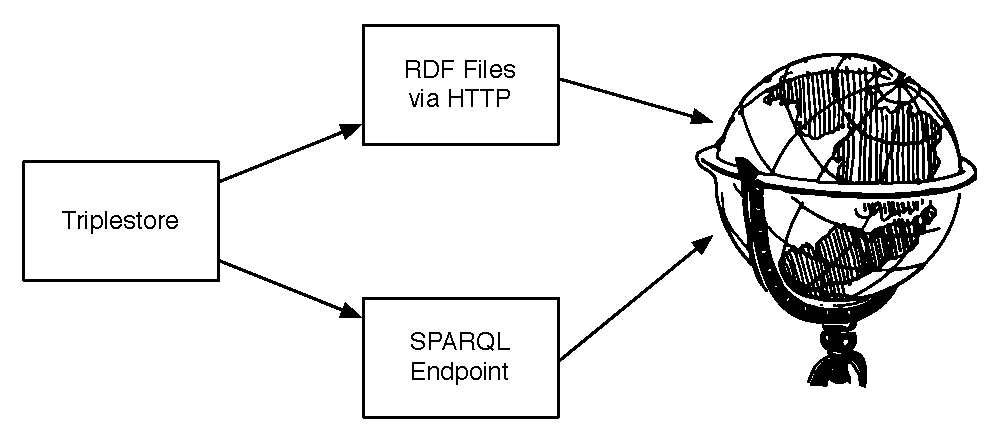
\includegraphics[scale=0.6,]{images/step1_2.pdf}
	\caption{Architektur: Daten veröffentlichen}
	\label{design-step12}
\end{figure}

\subsection{Joseki Server}
Die Joseki Web-Anwendung stellt das zentrale Element unseres Servers dar. Es erfüllt die Aufgabe, die gesammelten Daten dem gesamten Web bereit zu stellen. Unsere Anwendung (siehe \ref{cap-projektidee} und \ref{sec-our-app}) ist nur eine von vielen möglichen Anwendungen die diese Daten dann nutzen kann.

Da wir die Daten sowohl als statische RDF-Dateien zum Download, also auch über das SPARQL-Protokoll anbieten, werden die HTTP Verbindungen von einem Apache Webserver angenommen.
So werden die statischen Dateien, sowie die Beispiel-Webanwendung vom Apache ausgeliefert.
Stellt der Webserver anhand der aufgerufenen URL fest,
dass es sich um eine SPARQL Abfrage handelt, wird die Verbindung an den Joseki Server weitergegeben.

%\todo[inline]{Kurz die Config erklären, N3 usw. vielleicht auch die Storage Engines erwähnen?!}
%\todo[inline]{data.hs-weingarten.de ?? Oder erst in Fazit?}

\section{Die Anwendung: Semantic Internship Advisor}
\label{sec-our-app}

Die Anwendung wurde komplett in JavaScript realisiert. Dazu werden die beiden Bibliotheken ">jQuery"<\footnote{\url{http://jquery.com}} und ">sparql.js"< verwendet. Die Anwendung macht direkte Abfragen auf den Joseki SPARQL Endpoint (siehe \ref{sec-daten-joseki}).
Beim Aufruf der Anwendung werden die Themen und Schwerpunkte über eine SPARQL Abfrage geladen und daraus dynamisch eine HTML Form aufgebaut.
Hat der Benutzer seine Schwerpunkte und Präferenzen festgelegt werden die Firmen, die am ehesten dazu passen geladen und inklusive möglichen Betreuern angezeigt.

\paragraph{Abfragen}
In Listing \ref{umsetzung-app-sparql} ist zu sehen wie eine SPARQL Abfrage unter JavaScript aussehen kann.
In diesem Beispiel wird zuerst ein SPARQL Objekt mit dem Endpoint als Parameter angelegt.
Daraufhin werden wie üblich die verwendeten Namespaces deklariert.
In Zeile 7 wird das eigentliche Query ausgeführt, wobei wie in JavaScript üblich die Callback-Handler inline als Parameter angegeben werden.
Bei Erfolg (Zeile 13) kann die Antwort verarbeitet werden. Hier werden die einzelnen Schwerpunkte als Option in ein Auswahlfeld hinzugefügt.

\begin{lstlisting}[language=JavaScript,caption=SPARQL Abfrage mit JavaScript,stepnumber=1,label=umsetzung-app-sparql]
var s = new SPARQL.Service("http://fh-data.frubar.net/query/hswgt");
s.setPrefix("rdf", "http://www.w3.org/1999/02/22-rdf-syntax-ns#")
s.setPrefix("aiiso", "http://purl.org/vocab/aiiso/schema#")
s.setPrefix("dc", "http://purl.org/dc/elements/1.1/")

var q = s.createQuery();
q.query("SELECT ?m ?title FROM <http://fh-data.frubar.net/rdf/lsf.rdf> \
             WHERE { ?m rdf:type aiiso:Programme . ?m dc:title ?title }",
  {
    failure: function() {
      alert('Laden der Schwerpunkte fehlgeschlagen');
    },
    success: function(json) {
      for (var x in json.results.bindings) {
        $('#schwerpunkt').append($("<option></option>").
          attr("value",json.results.bindings[x].m.value).
          text(json.results.bindings[x].title.value));
      }
    }
  });
\end{lstlisting}

Folgende (geplante) Eigenschaften sind nicht implementiert:
\begin{itemize}
 \item Vorschlag eines Betreuers (Professor) pro Firma
 \item Daten vom LSF werden nicht verarbeitet
 \item Kein automatisches Laden von INKIDU Umfrageergebnissen
 \item Kein durchstöbern (browsen) der Daten möglich
% \item Keine LSF Integration der der Anwendung (als LSF-Modul)
\end{itemize}
Die Daten vom LSF konnten uns im Zeithorizont des Projektes leider Aufgrund von fehlenden Kapazitäten im Rechenzentrum nicht bereitgestellt werden.

\paragraph{Zuordnung} Die Zuordnung von Firmen zu den gewählten Schwerpunkten ist aus mehreren Gründen nicht wie in \ref{graphic-highlevel-data} beschreiben realisiert worden:
\begin{itemize}
 \item Keine ">echten"< Daten aus dem LSF.
 \item Fehlende Bewertung der Kriterien pro Veranstaltung
\end{itemize}

Aus diesen Gründen wurde für die Demo-Anwendung die Schwerpunkte direkt mit Kriterien (in der Anwendung Präferenzen genannt) bewertet. Diese Bewertung wurde von uns ">nach Gefühl"< vorgenommen.

Die Bewertungen werden aufgrund der in Abschnitt \ref{sec-algo} kurz angesprochenen Datenschutzbedenken nicht direkt veröffentlicht, sondern als ein Mittelwert. Daher wird auch nicht direkt der in \ref{klassifizierung} vorgestellte Nearest Neighbour Algorithmus verwendet. Das Prinzip ist zwar das selbe, jedoch gibt es für jede Klasse (entspricht Firma) nur einen Trainingsdatensatz. Somit werden diese nur aufsteigend nach den Abständen sortiert.

\begin{figure}[htbp]
	\centering
	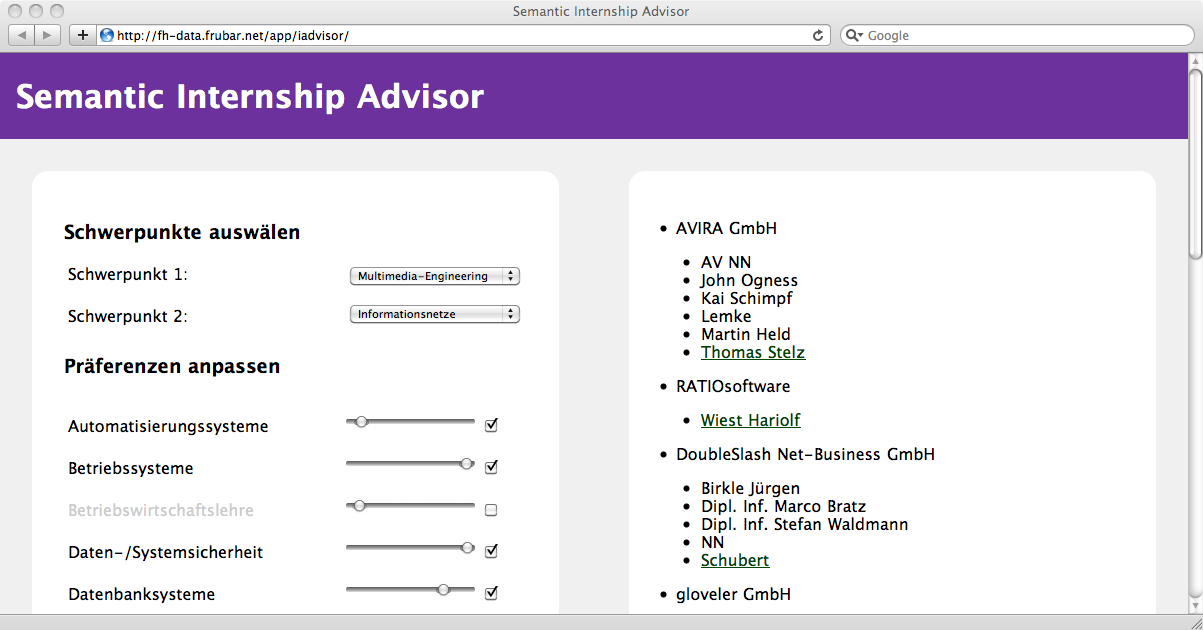
\includegraphics[scale=0.39]{images/sia.png}
	\caption{Screenshot der Anwendung }
	\label{sia-screenshot}
\end{figure}


\subsection{Semantische Benutzeroberflächen}
Da Semantic Web Anwendungen meist datenorientierter als herkömmliche Webanwendungen sind, sollten die Userinterface Möglichkeiten ebenfalls neu überdacht werden.
Für den Semantic Internship Advisor wird deshalb ein neues HTML5 Slider-Element verwendet um die Präferenzen einzustellen.
\begin{lstlisting}[language=HTML,caption=HTML 5 Slider,stepnumber=1,label=umsetzung-html5-slider]
<input type="range" />
\end{lstlisting}
Eine ausführlichere Betrachtung des Themas bietet \cite{Aufr08}.
Mit SMILE\footnote{\url{http://www.simile-widgets.org/}} gibt es bereits eine eigene Widget-Bibliothek für das Semantic Web.

Eine sehr frühe Demo-Version unserer Anwendung ist unter \url{http://fh-data.frubar.net/app/iadvisor/} zu finden.

\subsection{Mögliche Erweiterungen}

\paragraph{Maps} Es könnte z.B. aus den vorhandenen Adressdaten direkt ein Map-Widget eingebunden werden. APIs für diesen Zweck gibt es sowohl vom freien OpenStreetMaps (siehe Abbildung \ref{osm-screenshot}) als auch von Google.

\paragraph{Weitere Firmeninformationen} Es wäre denkbar über Freebase oder DBPedia (\ref{dbpedia}) Informationen wie ">Anzahl der Mitarbeiter"< abzufragen. Dabei gibt es nur ein Zuordnungsproblem. Gemäß dem Linked Data Ansatz müssten unsere RDFs eigentlich ein \textit{owl:sameAs} mit einer Referenz auf den Eintrag in z.B. DBPedia haben. Da wir diese Informationen jedoch nicht manuell nachtragen möchten, würde sich hier eine Suche nach Firmenname anbieten. SPARQL hilft dabei jedoch nicht, denn eine Freitextsuche ist hier (zumindest im Allgemeinen) nicht möglich. Es gibt jedoch Dienste wie \href{lookup.dbpedia.org}{http://lookup.dbpedia.org} die so etwas ermöglichen.

\begin{figure}[htbp]
	\centering
	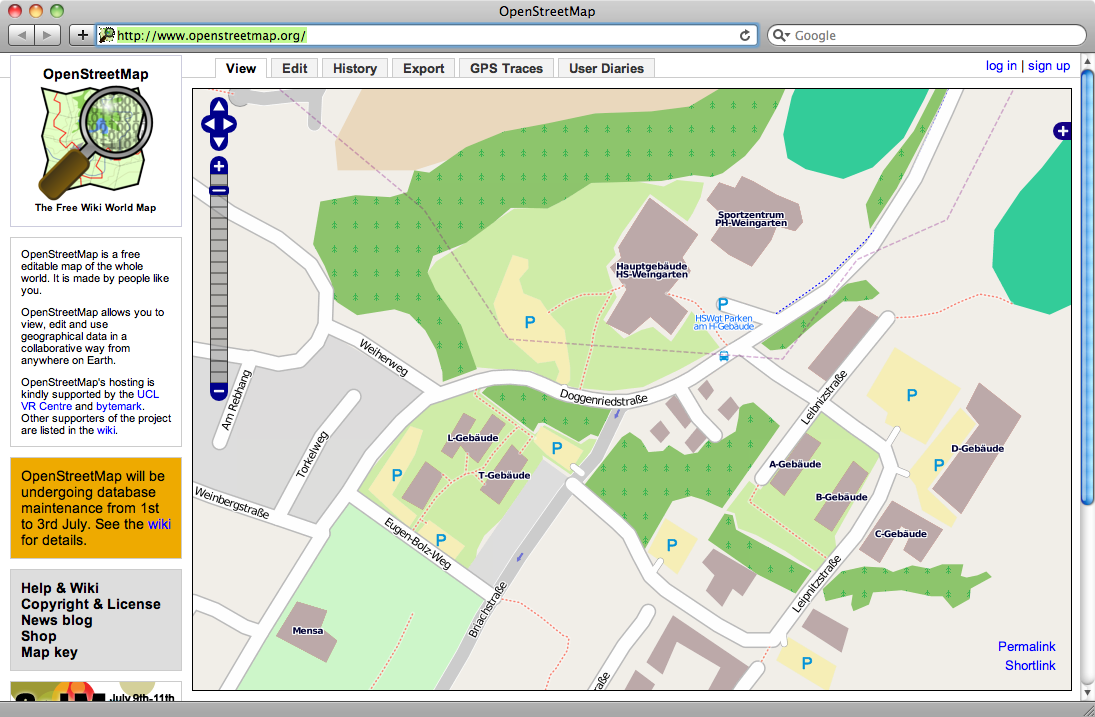
\includegraphics[scale=0.39]{images/osm-shot.png}
	\caption{OpenStreetMap Beispiel}
	\label{osm-screenshot}
\end{figure}


